\documentclass[UTF8]{article}
\usepackage{anyfontsize}
\usepackage{ctex}%中文
\usepackage{amsmath}
\usepackage{graphicx}%插图
\usepackage{bookmark}
\hypersetup{hidelinks}
\usepackage{amstext}%数学环境中的文字
\usepackage{esint}%曲面积分符号
\usepackage{eucal}%特殊数学字体
\usepackage{geometry}
\usepackage{tikz}
\usetikzlibrary{patterns}

\geometry{a4paper,scale=0.8}


\begin{document}
\title{电动力学}
\author{zhufeng}
\date{}
\maketitle
\tableofcontents
\newpage
\section{准备知识}
\subsection{散度和旋度}
散度定理(1)和旋度定理(2):
\begin{align}
    \oiint F dS = \int_V \nabla \cdot F dV \\
    \oint F dl = \int _S \nabla\times F dS
\end{align}
\subsection{格林定理}
由散度定理导出,设矢量函数由两个标量函数组成$F = \varphi \nabla \psi$,将这个式子代入
(1)得到:
\begin{align}
    \int _V (\varphi\nabla^2\psi+\nabla \varphi\cdot \nabla \psi) dV = \oint \varphi
    \frac{\partial \psi}{\partial n}dS
\end{align}
公式(3)为格林第一恒等式,继续假设$F = \psi \nabla \varphi$,代入(1):
\begin{align}
    \int _V (\psi\nabla^2\varphi+\nabla \psi\cdot \nabla \varphi) dV = \oint \psi
    \frac{\partial \varphi}{\partial n}dS
\end{align}
方程(4)-方程(3):
\begin{align}
    \int( \psi\nabla^2\varphi-\varphi\nabla^2\psi) dV = \oint  (\psi
    \frac{\partial \varphi}{\partial n}-\varphi\frac{\partial \psi}{\partial n}) dS
\end{align}
方程(5)为格林第二恒等式。
\subsection{亥姆霍兹定理}
在有限区域V内,任意矢量场可以由其散度,旋度以及边界条件表示:
\begin{align}
    F(r)=\-\nabla \mu(r) + \nabla\times A
\end{align}
\subsection{电磁场的基本规律}
麦克斯韦方程组的积分形式(3)和微分形式(4):
\begin{align}
    \begin{cases}
        \oiint D dS  =\iiint \rho dV                        \\
        \oiint B dS =0                                      \\
        \oint  E dl =\iint -\frac{\partial B}{\partial t}dS \\
        \oint H dl=\iint JdS+\iint \frac{\partial D}{\partial t}dS
    \end{cases}
\end{align}
\begin{align}
    \begin{cases}
        \nabla \cdot D  =\rho                           \\
        \nabla \cdot B  =0                              \\
        \nabla \times E =-\frac{\partial B}{\partial t} \\
        \nabla \times H =J+\frac{\partial D}{\partial t}
    \end{cases}
\end{align}


当有媒介存在时,上述方程组还是不够完备的,对于各向同性和线性的媒介,还需要
满足:
\begin{align}
    J = \sigma E,D = \varepsilon E ,H = \frac{B}{\mu}
\end{align}

\subsection{电磁场的边界条件}
在不同媒介的分界面上,某些场的分量发生突变,微分形式的麦克斯韦方程组反应的
是某一点的场的特征,因此此时需要用到积分形式的麦克斯韦方程组来确定边界
条件(如图2.7.1):
\begin{align}
    \oint H dl =\int _S JdS \Rightarrow 
    \int _{ab} H_1 (e_S\times e_n)dl +\int _{cd} H_2(e_S\times e_n)dl
    =\int _S J \cdot e_S dS \\
    \oint e_n\times (H_2-H_1) \cdot e_S dl
    = \int _S J \cdot e_S dS \Rightarrow e_n\times(H_2-H_1)=J
\end{align}
类似的求法我们可以得到这样一组边界条件:
\begin{align}
    &e_n \times (H_2-H_1) = J \\
    &e_n \cdot (B_2-B_1)=0    \\
    &e_n \times (E_2-E_1)=0   \\
    &e_n \cdot (D_2-D_1)=\rho
\end{align}
\newpage
\section{势能}
\subsection{镜像法}
\begin{figure}[htbp]
\centering
\tikzset{every picture/.style={line width=0.75pt}} %set default line width to 0.75pt        
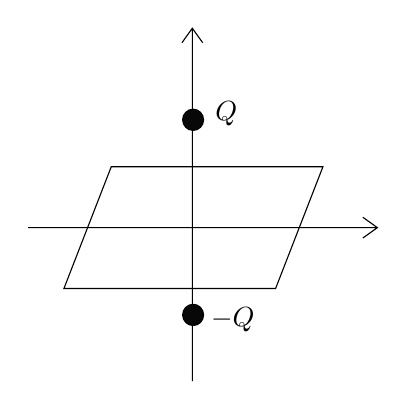
\begin{tikzpicture}[x=0.75pt,y=0.75pt,yscale=-1,xscale=1]
%uncomment if require: \path (0,300); %set diagram left start at 0, and has height of 300

%Shape: Rectangle [id:dp539416937811162] 
\draw   (247.99,170.25) -- (349.98,170.25) -- (327.17,228.92) -- (225.19,228.92) -- cycle ;
%Shape: Axis 2D [id:dp5302013943533057] 
\draw  (208,199.58) -- (376.22,199.58)(287.06,103.5) -- (287.06,273.56) (369.22,194.58) -- (376.22,199.58) -- (369.22,204.58) (282.06,110.5) -- (287.06,103.5) -- (292.06,110.5)  ;
%Flowchart: Connector [id:dp12314201247187362] 
\draw  [fill={rgb, 255:red, 8; green, 8; blue, 8 }  ,fill opacity=1 ] (282.39,147.62) .. controls (282.39,150.44) and (284.65,152.72) .. (287.44,152.72) .. controls (290.23,152.72) and (292.48,150.44) .. (292.48,147.62) .. controls (292.48,144.8) and (290.23,142.52) .. (287.44,142.52) .. controls (284.65,142.52) and (282.39,144.8) .. (282.39,147.62) -- cycle ;
%Flowchart: Connector [id:dp07621270965246985] 
\draw  [fill={rgb, 255:red, 8; green, 8; blue, 8 }  ,fill opacity=1 ] (282.39,241.62) .. controls (282.39,244.44) and (284.65,246.72) .. (287.44,246.72) .. controls (290.23,246.72) and (292.48,244.44) .. (292.48,241.62) .. controls (292.48,238.8) and (290.23,236.52) .. (287.44,236.52) .. controls (284.65,236.52) and (282.39,238.8) .. (282.39,241.62) -- cycle ;
% Text Node
\draw (296.89,137.51) node [anchor=north west][inner sep=0.75pt]    {$Q$};
% Text Node
\draw (294.89,236.84) node [anchor=north west][inner sep=0.75pt]    {$-Q$};
\end{tikzpicture}
\end{figure}
如图所示的平板是接地的,$V=0$,并且在无穷远处,$V=0$,如果要求出任意点的电势,
除了考虑点电荷还需要考虑平板产生的感应电荷,这两个电荷产生的电势叠加就是上半部分
任意点的电势,根据唯一性原理,在平板下面放置一个-Q的电荷然后去掉平板可以产生
一样的效果,下半区虽然不一样,但是我们并不关心这块地方的电势究竟是怎么样的。
因此,可以得到上半平面的电势为:
\begin{align*}
    V = \frac{1}{4\pi \varepsilon_0 }(\frac{Q}{r}+\frac{-Q}{r'})
\end{align*}

另外一个例子:
\begin{figure}[htbp]
\centering
% Pattern Info
\tikzset{
pattern size/.store in=\mcSize, 
pattern size = 5pt,
pattern thickness/.store in=\mcThickness, 
pattern thickness = 0.3pt,
pattern radius/.store in=\mcRadius, 
pattern radius = 1pt}
\makeatletter
\pgfutil@ifundefined{pgf@pattern@name@_5aqoundks}{
\makeatletter
\pgfdeclarepatternformonly[\mcRadius,\mcThickness,\mcSize]{_5aqoundks}
{\pgfpoint{-0.5*\mcSize}{-0.5*\mcSize}}
{\pgfpoint{0.5*\mcSize}{0.5*\mcSize}}
{\pgfpoint{\mcSize}{\mcSize}}
{
\pgfsetcolor{\tikz@pattern@color}
\pgfsetlinewidth{\mcThickness}
\pgfpathcircle\pgfpointorigin{\mcRadius}
\pgfusepath{stroke}
}}
\makeatother

% Pattern Info
 
\tikzset{
pattern size/.store in=\mcSize, 
pattern size = 5pt,
pattern thickness/.store in=\mcThickness, 
pattern thickness = 0.3pt,
pattern radius/.store in=\mcRadius, 
pattern radius = 1pt}
\makeatletter
\pgfutil@ifundefined{pgf@pattern@name@_xm9iz4hxz}{
\makeatletter
\pgfdeclarepatternformonly[\mcRadius,\mcThickness,\mcSize]{_xm9iz4hxz}
{\pgfpoint{-0.5*\mcSize}{-0.5*\mcSize}}
{\pgfpoint{0.5*\mcSize}{0.5*\mcSize}}
{\pgfpoint{\mcSize}{\mcSize}}
{
\pgfsetcolor{\tikz@pattern@color}
\pgfsetlinewidth{\mcThickness}
\pgfpathcircle\pgfpointorigin{\mcRadius}
\pgfusepath{stroke}
}}
\makeatother

% Pattern Info
 
\tikzset{
pattern size/.store in=\mcSize, 
pattern size = 5pt,
pattern thickness/.store in=\mcThickness, 
pattern thickness = 0.3pt,
pattern radius/.store in=\mcRadius, 
pattern radius = 1pt}
\makeatletter
\pgfutil@ifundefined{pgf@pattern@name@_4ruiz8ncj}{
\makeatletter
\pgfdeclarepatternformonly[\mcRadius,\mcThickness,\mcSize]{_4ruiz8ncj}
{\pgfpoint{-0.5*\mcSize}{-0.5*\mcSize}}
{\pgfpoint{0.5*\mcSize}{0.5*\mcSize}}
{\pgfpoint{\mcSize}{\mcSize}}
{
\pgfsetcolor{\tikz@pattern@color}
\pgfsetlinewidth{\mcThickness}
\pgfpathcircle\pgfpointorigin{\mcRadius}
\pgfusepath{stroke}
}}
\makeatother

% Pattern Info
 
\tikzset{
pattern size/.store in=\mcSize, 
pattern size = 5pt,
pattern thickness/.store in=\mcThickness, 
pattern thickness = 0.3pt,
pattern radius/.store in=\mcRadius, 
pattern radius = 1pt}
\makeatletter
\pgfutil@ifundefined{pgf@pattern@name@_qtnq7w0c2}{
\makeatletter
\pgfdeclarepatternformonly[\mcRadius,\mcThickness,\mcSize]{_qtnq7w0c2}
{\pgfpoint{-0.5*\mcSize}{-0.5*\mcSize}}
{\pgfpoint{0.5*\mcSize}{0.5*\mcSize}}
{\pgfpoint{\mcSize}{\mcSize}}
{
\pgfsetcolor{\tikz@pattern@color}
\pgfsetlinewidth{\mcThickness}
\pgfpathcircle\pgfpointorigin{\mcRadius}
\pgfusepath{stroke}
}}
\makeatother

% Pattern Info
 
\tikzset{
pattern size/.store in=\mcSize, 
pattern size = 5pt,
pattern thickness/.store in=\mcThickness, 
pattern thickness = 0.3pt,
pattern radius/.store in=\mcRadius, 
pattern radius = 1pt}
\makeatletter
\pgfutil@ifundefined{pgf@pattern@name@_zmoklyqzv}{
\makeatletter
\pgfdeclarepatternformonly[\mcRadius,\mcThickness,\mcSize]{_zmoklyqzv}
{\pgfpoint{-0.5*\mcSize}{-0.5*\mcSize}}
{\pgfpoint{0.5*\mcSize}{0.5*\mcSize}}
{\pgfpoint{\mcSize}{\mcSize}}
{
\pgfsetcolor{\tikz@pattern@color}
\pgfsetlinewidth{\mcThickness}
\pgfpathcircle\pgfpointorigin{\mcRadius}
\pgfusepath{stroke}
}}
\makeatother

% Pattern Info
 
\tikzset{
pattern size/.store in=\mcSize, 
pattern size = 5pt,
pattern thickness/.store in=\mcThickness, 
pattern thickness = 0.3pt,
pattern radius/.store in=\mcRadius, 
pattern radius = 1pt}
\makeatletter
\pgfutil@ifundefined{pgf@pattern@name@_qbnleqbz0}{
\makeatletter
\pgfdeclarepatternformonly[\mcRadius,\mcThickness,\mcSize]{_qbnleqbz0}
{\pgfpoint{-0.5*\mcSize}{-0.5*\mcSize}}
{\pgfpoint{0.5*\mcSize}{0.5*\mcSize}}
{\pgfpoint{\mcSize}{\mcSize}}
{
\pgfsetcolor{\tikz@pattern@color}
\pgfsetlinewidth{\mcThickness}
\pgfpathcircle\pgfpointorigin{\mcRadius}
\pgfusepath{stroke}
}}
\makeatother

% Pattern Info
 
\tikzset{
pattern size/.store in=\mcSize, 
pattern size = 5pt,
pattern thickness/.store in=\mcThickness, 
pattern thickness = 0.3pt,
pattern radius/.store in=\mcRadius, 
pattern radius = 1pt}
\makeatletter
\pgfutil@ifundefined{pgf@pattern@name@_y4adkcgg1}{
\makeatletter
\pgfdeclarepatternformonly[\mcRadius,\mcThickness,\mcSize]{_y4adkcgg1}
{\pgfpoint{-0.5*\mcSize}{-0.5*\mcSize}}
{\pgfpoint{0.5*\mcSize}{0.5*\mcSize}}
{\pgfpoint{\mcSize}{\mcSize}}
{
\pgfsetcolor{\tikz@pattern@color}
\pgfsetlinewidth{\mcThickness}
\pgfpathcircle\pgfpointorigin{\mcRadius}
\pgfusepath{stroke}
}}
\makeatother
\tikzset{every picture/.style={line width=0.75pt}} %set default line width to 0.75pt        

\begin{tikzpicture}[x=0.75pt,y=0.75pt,yscale=-1,xscale=1]
%uncomment if require: \path (0,300); %set diagram left start at 0, and has height of 300

%Shape: Axis 2D [id:dp18747467408618257] 
\draw  (203.56,170.44) -- (303.56,170.44)(249.56,102.44) -- (249.56,229.78) (296.56,165.44) -- (303.56,170.44) -- (296.56,175.44) (244.56,109.44) -- (249.56,102.44) -- (254.56,109.44)  ;
%Straight Lines [id:da9502279074682827] 
\draw [pattern=_5aqoundks,pattern size=6pt,pattern thickness=0.75pt,pattern radius=0.75pt, pattern color={rgb, 255:red, 0; green, 0; blue, 0}]   (249.56,140.88) -- (251.74,140.88) ;
%Straight Lines [id:da40366396117791803] 
\draw [pattern=_xm9iz4hxz,pattern size=6pt,pattern thickness=0.75pt,pattern radius=0.75pt, pattern color={rgb, 255:red, 0; green, 0; blue, 0}]   (251.74,140.88) -- (253.93,140.88) ;
%Straight Lines [id:da13596137932234464] 
\draw [pattern=_4ruiz8ncj,pattern size=6pt,pattern thickness=0.75pt,pattern radius=0.75pt, pattern color={rgb, 255:red, 0; green, 0; blue, 0}]   (253.93,140.88) -- (256.11,140.88) ;
%Straight Lines [id:da16660170966964927] 
\draw [pattern=_qtnq7w0c2,pattern size=6pt,pattern thickness=0.75pt,pattern radius=0.75pt, pattern color={rgb, 255:red, 0; green, 0; blue, 0}]   (256.11,140.88) -- (258.3,140.88) ;
%Straight Lines [id:da5222395126935209] 
\draw [pattern=_zmoklyqzv,pattern size=6pt,pattern thickness=0.75pt,pattern radius=0.75pt, pattern color={rgb, 255:red, 0; green, 0; blue, 0}]   (258.3,140.88) -- (260.48,140.88) ;
%Straight Lines [id:da8846993806890491] 
\draw [pattern=_qbnleqbz0,pattern size=6pt,pattern thickness=0.75pt,pattern radius=0.75pt, pattern color={rgb, 255:red, 0; green, 0; blue, 0}]   (260.48,140.88) -- (262.67,140.88) ;
%Straight Lines [id:da3808194430157834] 
\draw [pattern=_y4adkcgg1,pattern size=6pt,pattern thickness=0.75pt,pattern radius=0.75pt, pattern color={rgb, 255:red, 0; green, 0; blue, 0}]   (262.67,140.88) -- (269.22,140.88) -- (275.78,140.88) -- (282.33,140.89) -- (288.89,140.89) ;
%Straight Lines [id:da8832899784206474] 
\draw    (288.89,140.89) -- (288.89,172.89) ;
%Straight Lines [id:da6189396516724448] 
\draw    (249.56,140.88) -- (210.89,140.88) ;
%Straight Lines [id:da22484186565745556] 
\draw    (288.89,199.79) -- (248.89,199.54) ;
%Straight Lines [id:da41997799859034646] 
\draw    (248.89,199.54) -- (210.22,199.54) ;
%Straight Lines [id:da13037138591742026] 
\draw    (210.89,167.78) -- (210.89,140.88) ;
%Straight Lines [id:da907289938374868] 
\draw    (210.22,199.54) -- (210.89,167.78) ;
%Straight Lines [id:da6011175293362048] 
\draw    (288.89,199.79) -- (288.89,187.11) -- (288.89,172.89) ;

% Text Node
\draw (286.89,123.84) node [anchor=north west][inner sep=0.75pt]  [xscale=1.5,yscale=1.5]  {$Q$};
% Text Node
\draw (185.56,124.07) node [anchor=north west][inner sep=0.75pt]  [xscale=1.5,yscale=1.5]  {$-Q$};
% Text Node
\draw (285.56,194.93) node [anchor=north west][inner sep=0.75pt]  [xscale=1.5,yscale=1.5]  {$-Q$};
% Text Node
\draw (193.56,197.07) node [anchor=north west][inner sep=0.75pt]  [xscale=1.5,yscale=1.5]  {$Q$};


\end{tikzpicture}
\end{figure}
在第一象限存在一个电荷Q,x和y平板的电势为0,那么利用这个条件,去掉平板,加入电荷
以得到相同的边界条件,可以求出第一象限的任一点的电势为:
\begin{align*}
     &(-a,b),(-a,-b),(a,b),(a,-b)\\
     V = \frac{1}{4\pi \varepsilon_0}(
    &\frac{-Q}{\sqrt{(x+a)^2+(y-b)^2}}
     +\frac{Q}{\sqrt{(x-a)^2+(y-b)^2}}\\
     &+\frac{-Q}{\sqrt{(x-a)^2+(y+b)^2}}+\frac{Q}{\sqrt{(x+a)^2+(y+b)^2}})
\end{align*}


\newpage
\section{静磁场及其边值问题的解}
\section{时变电磁场}
\subsection{磁矢势和规范不变性}
前面我们使用标量函数来表示电场,由于此时电场的旋度不为零,不能只是使用
标量函数的额梯度来表示,这里我们使用矢量位A和标量位$\varphi$来表示:
\begin{align}
    &B=\nabla \times A\\
    &\nabla \times E = -\nabla \times \frac{\partial A}{\partial t}\\
    & \nabla \times(E+\frac{\partial A}{\partial t})=0\Rightarrow E
    +\frac{\partial A}{\partial t}=-\nabla \varphi
\end{align}
E可以使用A和一个标量函数来表示,B可以用A来表示,由于规范不变性:
\begin{align}
    \begin{cases}
        A' = A + \nabla \psi \\
        \varphi' = \varphi - \frac{\partial \psi}{\partial t}
    \end{cases}
\end{align}
这样的A和$\psi$有无数组,为了确定它,使用洛伦兹规范:
\begin{align}
    \nabla \cdot A = \mu\varepsilon \frac{\partial \psi}{\partial t}
\end{align}
\subsection{达朗贝尔方程}
波动方程:
\begin{align}
    \begin{cases}
        \nabla^2H-\mu\varepsilon \frac{\partial^2 H}{\partial t^2}=0 \\
        \nabla^2E-\mu\varepsilon \frac{\partial^2 E}{\partial t^2}=0 \\
    \end{cases}
\end{align}
结合方程(8)和(18),得到达朗贝尔方程:
\begin{align}
    \nabla^2 A -\mu\varepsilon \frac{\partial^2 A}{\partial t^2}=-\mu J\\
    \nabla^2 \varphi -\mu\varepsilon \frac{\partial^2 \varphi}{\partial t^2}=-\frac{\rho}{\varepsilon}
\end{align}
\subsection{坡印廷矢量}

\subsection{时谐电磁波}
时谐波的数学形式:
\begin{gather}
    \begin{cases}
        E\left( x,t \right) =E\left( x \right) e^{-i(\omega t+\phi(x))} \\
        H\left( x,t \right) =H\left( x \right) e^{-i(\omega t+\phi(x))} 
    \end{cases}
\end{gather}
\subsection{复矢量的麦克斯韦方程组}
如果时谐电磁场的解可以使用$u(r)=u_{m(r)}e^{i(\omega t +\phi(r))}$表示,则此时的麦克斯韦方程组
可以简化为:
\begin{align}
    \begin{cases}
        \nabla \cdot D  =\rho                           \\
        \nabla \cdot B  =0                              \\
        \nabla \times E =-i\omega B \\
        \nabla \times H =J+i\omega D
    \end{cases}
\end{align}
\subsection{复电容率和复磁导率}
首先推导复电容率,然后根据类比得到复磁导率:
\begin{align}
    &\nabla \times H = J + \varepsilon \frac{\partial E}{\partial t}\\
    &\nabla \times H = \sigma E +i \varepsilon \omega E\\
    &\nabla \times H = i\omega(\varepsilon-i\frac{\sigma}{\omega})E
\end{align}
则根据式(26)可以得到复电容率(电介质常数)(类似的有复磁导率):
\begin{align}
    \varepsilon' = \varepsilon -i(\frac{\sigma}{\omega}+\varepsilon'')\\
    \mu' = \mu -i\mu''
\end{align}
导电媒介的损耗均以复虚数的形式表示出来,例如在式(27)中,$\sigma/\omega$表示的是欧姆损耗,$\varepsilon''$表示
的是电极化损耗,式(27)中$\mu''$表示的是磁化损耗。
\subsection{亥姆霍兹方程}
我们将时谐场解的形式代入(21)可以得到亥姆霍兹方程:
\begin{align}
    \begin{cases}
        \nabla^2 B + \mu \varepsilon \omega^2 B = 0\\
        \nabla^2 E + \mu \varepsilon \omega^2 E = 0
    \end{cases}
\end{align}
\section{均匀平面波在无界空间中的传播}
\subsection{理想介质中的传播}
理想介质中没有损耗存在,$E_Z=H_Z=0$,这个东西需要思考一下,延着Z轴传播的的电场X轴上的分量为$E_x(z,t)$,这个分量
可以写成时谐波的形式:
\begin{align}
    E_x(z,t)=E_{xm}e^{i(\omega t -kz+\phi)}
\end{align}
波阻抗反映了E和H是否同相位,如果波阻抗是复数,那么磁场将会附加一段相位,导致两者的相位是不相同的。
\subsection{真空中的平面单色波}
由于真空中的电磁波没有电流源和电荷源,因此根据麦克斯韦方程组:
\begin{align*}
    \begin{array}{l}  
     \nabla \cdot \mathbf{E} =\cfrac{\rho}{\varepsilon _0}  \\  
     \nabla \cdot \mathbf{B} = 0 \\  
     \nabla \times  \mathbf{E} = -\cfrac{\partial \mathbf{B}}{\partial t }  \\  
     \nabla \times  \mathbf{B} = \mu _0(\mathbf{J} + \varepsilon_0 \cfrac{\partial \mathbf{E}}{\partial t }  )
 \end{array}  
 \end{align*}
前面已经知道平面单色波的波函数的形式:
\begin{align*}
    &E = E_{m} e^{i(\omega t- ky)}\\
    &B = B_{m} e^{i(\omega t- ky)}
\end{align*}
假设E和B的传播方向都是延着y轴,将上述波函数代入麦克斯韦方程组的前两个可以得到:
\begin{align*}
    &E_y = 0 \qquad B_y = 0\\
    &\frac{\partial E_z}{\partial y}-\frac{\partial E_y}{\partial z} =
     -\frac{\partial B_x}{\partial t}\\
     &\frac{\partial E_y}{\partial x}-\frac{\partial E_x}{\partial y} =
     -\frac{\partial B_z}{\partial t}
\end{align*}
解上面这个方程组可以得到E和B的关系:
\begin{align*}
    &E _{zm} = \frac{\omega}{k}B_{xm}\qquad E_{xm} = -\frac{\omega}{k}B_{zm}\\
    &\mathbf{ B} = \frac{\omega}{k} \mathbf{y} \times \mathbf{E} 
\end{align*}
\subsection{导电媒介中的传播}
在导电媒介中传播时,是存在损耗的,在()节时,三种损耗所引起的变为复数的电介质常数和磁介质常数,会导致原本的时谐波中会多出一个表示
衰减的e指数项,因此会产生趋肤效应,关于趋肤效应的具体解释:
\subsection{良导体中的传播}
良导体所满足的条件:$\frac{\sigma}{\mu \varepsilon}>>1$,根据近似,得出电磁波在良导体中的传播特性:

\subsection{弱导电媒介中传播}
弱导电媒介所满足的条件:$\frac{\sigma}{\mu \varepsilon}<<1$,根据近似,得出电磁波在弱导电媒介中的传播特性:

\subsection{电磁波的极化}
极化:由于$E_x,E_y$的相位的振幅不一定相同,这就导致了叠加后的电场大小和方向都有可能随时间变化,这
种现象被称为电磁波的极化。
假设:
\begin{align}
    E_x = E_{xm} \cos(\omega t +\phi_1)\\
    E_y = E_{ym} \cos(\omega t +\phi_2)
\end{align}
三种极化波分别是:线极化波$(\Delta \phi =0, \pm \pi)$,圆极化波$(\Delta \phi = \pm\frac{\pi}{2})$且振幅相同,椭圆极化波(振幅和相位均不相等)。\\
\textbf{线极化波:}
\begin{align}
    E = \sqrt{(E_{xm})^2+(E_{ym})^2}\cos (\omega t+\phi_1)
\end{align}
应用:信号发射的电场方向应该与信号接收者天线的方向平行。垂直极化波和平行
极化波(垂直于地面的为垂直极化波,平行于地面的为平行极化波)\\
\textbf{圆极化波:}
\begin{align}
    (E_x)^2+(E_y)^2=E_m^2
\end{align}
应用:在火箭上发射的信号为圆极化波,在各个方向上的电场均有振幅,如果改为
线极化波,则有可能导致火箭无法收到信号而导致失控。(左旋圆极化波和右旋圆极
化波,传播方向和矢量旋转方向满足右手法则,则为右旋,否则则为左旋)\\
\textbf{椭圆极化波:}
\begin{align}
    \frac{E_x^2}{E_{xm}^2}+\frac{E_y^2}{E_{ym}^2}-\frac{2E_xE_y}{E_{xm}E_{ym}}
    \cos \phi =\sin \phi
\end{align}
应用:关于左旋椭圆极化波和右旋椭圆极化波的判断和圆极化波类似(当观察者朝向电磁波的方向时,如果电场向量按逆时针方向旋转,则为左旋圆极化波;
如果电场向量按顺时针方向旋转,则为右旋圆极化波,这是从另外一种角度判断)。线和圆极化波
是椭圆极化波的特例。
\subsection{色散与群速}
首先需要了解什么是色散介质:相速度的定义:
$$v_p = \frac{\omega}{k}$$
当$\omega$和$k$不在构成线性关系,电磁波的相速随频率改变,产生色散现象。

信号是由许许多多的频率的电磁波组成的,稳定的单一频率的波不携带任何信息,因此用相速度
并不能描述信号在媒介中的传播速度,此时需要使用群速的概念:包络波上任意一点的
相位的推进速度。例如:
\begin{align}
    &E = 2E_m \cos (\Delta \omega t - \Delta k z) e^{-i(\omega t -k z)}\\
    &v_g = \frac{d\omega}{dk}
\end{align}

\section{均匀平面的波的反射与透射}
\subsection{电磁波在介质面上的反射与折射}
经过我看书之梳理一遍之后,发现数理方法真的好重要,现在没事就要看看数理方法的书,才行!!!
一般情况下的电磁场的边值关系:
$$
    \begin{array}{l}
        e_{ n } \times\left( E _{2}- E _{1}\right)=0       \\
        e_{ n } \times\left( H _{2}- H _{1}\right)= \alpha \\
        e _{ n } \cdot\left( D _{2}- D _{1}\right)=\sigma  \\
        e _{ n } \cdot\left( B _{2}- B _{1}\right)=0
    \end{array}
$$
由于之前我们推导的时谐波的麦克斯韦方程组四个不是独立的,可以由其中的两个推得另外的两个,因此在介质的情况下我们仅需
\begin{align*}
    e_n\times(E_2-E_1)=0 \\
    e_n\times (H_2-H_1)=0
\end{align*}
$k,k',k''$为波矢量,平面波的表达式分别为:
$$
    \begin{array}{l}
        E = E _{0} e ^{ i (k \cdot x-\omega t)}                                         \\
        E ^{\prime}= E _{0}^{\prime} e ^{ i \left( k ^{\prime} \cdot x-\omega t\right)} \\
        E ^{\prime \prime}= E _{0}^{\prime \prime} e ^{ i \left( K ^{\prime} \cdot x-\omega t\right)}
    \end{array}
$$
入射前的场强叠加和入射后的场强叠加应该是一样的:
\begin{align*}
    e_n\times = (E+E')=e_n\times E''
\end{align*}
代入前面的时谐波形式,
可以得到:
\begin{align*}
    k\cdot x=k' \cdot x=k''\cdot x
\end{align*}
因为k是矢量,则对应的分量应该是相等的。
\begin{center}
    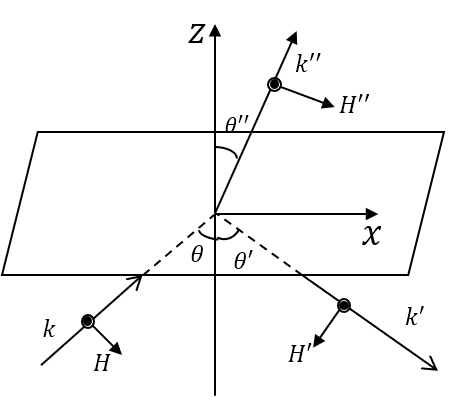
\includegraphics[scale=0.7]{img/fanshe.png}
\end{center}

如图所示,对相应的分量进行分析:
\begin{align*}
    k_x   & =k\sin \theta      \\
    k_x'  & =k'\sin \theta'    \\
    k_x'' & =k'' \sin \theta''
\end{align*}
又$k=k'=\frac{\omega}{v_1},k''=\frac{\omega}{v_2}$,可以得到反射定律和折射定律,
\begin{align*}
    \theta =\theta ',\frac{\sin \theta}{\sin \theta''}=\frac{v_1}{v_2}
\end{align*}
还可以得到折射率和反射角与入射角的关系:
\begin{align*}
    \frac{\sin \theta}{\sin \theta''}=\frac{n_2}{n_1}=\frac{\sqrt{\mu_2\varepsilon_2}}{\sqrt{\mu_1\varepsilon_1}}=\frac{\varepsilon_2}{\varepsilon_1}
\end{align*}
接下来根据第二个方程推得菲涅尔公式,根据如图所示的情况:既第一种情况E和入射面垂直
\begin{align*}
    H\cos  \theta -H'\cos\theta'=H''\cos \theta''
\end{align*}
$$
    \sqrt{\varepsilon_{1}}\left(E-E^{\prime}\right) \cos \theta=\sqrt{\varepsilon_{2}} E^{\prime \prime} \cos \theta^{\prime \prime}
$$
并由折射定律得:
$$
    \begin{array}{l}
        \dfrac{E^{\prime}}{E}=\dfrac{\sqrt{\varepsilon_{1}} \cos \theta-\sqrt{\varepsilon_{2}} \cos \theta^{\prime \prime}}{\sqrt{\varepsilon_{1}} \cos \theta+\sqrt{\varepsilon_{2}} \cos \theta^{\prime \prime}}=-\dfrac{\sin \left(\theta-\theta^{\prime \prime}\right)}{\sin \left(\theta+\theta^{\prime \prime}\right)} \\[0.5cm]
        \dfrac{E^{\prime \prime}}{E}=\dfrac{2 \sqrt{\varepsilon_{1}} \cos \theta}{\sqrt{\varepsilon_{1}} \cos \theta+\sqrt{\varepsilon_{2}} \cos \theta^{\prime \prime}}=\dfrac{2 \cos \theta \sin \theta^{\prime \prime}}{\sin \left(\theta+\theta^{\prime \prime}\right)}
    \end{array}
$$
另外一种情况E与入射面平行的情况,和上图类似,就是H和E换一个位置:
\section{狭义相对论}
迈克耳孙-莫雷实验证明了光速不变理论
\begin{center}
    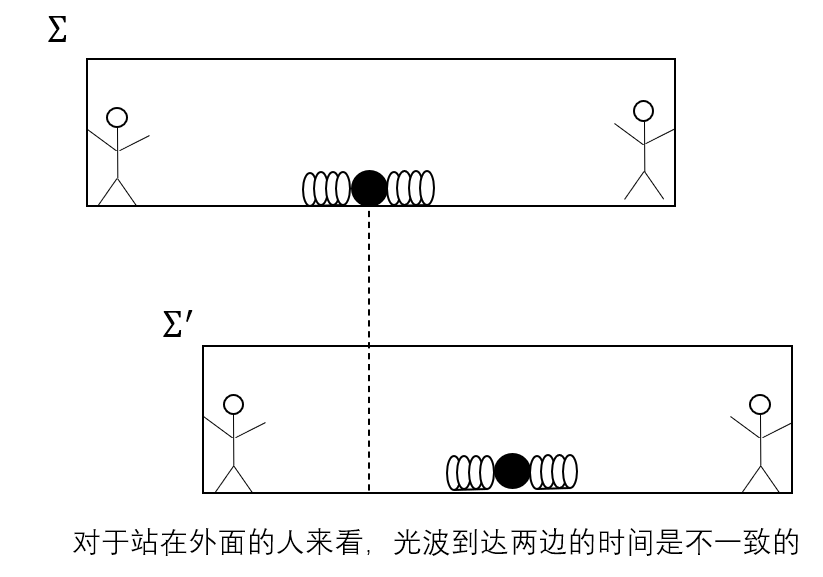
\includegraphics[scale=0.7]{img/xiaxiang.png}
\end{center}
伽利略变换仅适用于宏观低速的情况,但是在电磁理论当中,c是不变量,不符合伽利略变换。
狭义相对论的两大研究问题:1,相对论原理,2,光速不变理论
\subsection{洛伦兹变换}
事件间隔不变性,r是物体走过的距离:以光信号连接时$r^2=c^2t^2$,不是以光信号连接时:$r^2<c^2t^2$。
两个事件间隔:时间坐标和空间坐标联系到一起:
\begin{align*}
    S'=c^2(t_1'-t_2')^2-[(x_2'-x_1')^2+(y_2'-y_1')^2+(z_2'-z_1')^2] \\
    S=c^2(t_1-t_2)^2-[(x_2-x_1)^2+(y_2-y_1)^2+(z_2-z_1)^2]
\end{align*}
其中S和$S'$是表示的事件间隔,我们类比于空间坐标的间隔:
\begin{align*}
    r^2=(x_2-x_1)^2+(y_2-y_1)^2+(z_2-z_1)^2
\end{align*}
但是对于为什么多了时间项,原因肯定是多了一个时间坐标,又时间坐标的平方和空间坐标相差一个符号,原因就是时间项含有虚数。因此对于四维矢量,我们可以写成如下形式:
\begin{align*}
    (x_1,x_2,x_3,ict)
\end{align*}

\end{document}